\section{Introduction}
\label{sec:intro}

%% datacenter is high impact topic 
Data centers (\DCs) are a critical piece of today's networked applications in
both private~\cite{} and  public sectors~\cite{}.   The key
factors that have driven this trend  are  economies of scale, 
   reduced  management costs, better utilization of hardware
via statistical multiplexing, and the ability to elastically
scale applications in response to changing workload patterns.  

%
%% datacenter network needs to be designed carefully
A robust  {\em datacenter network fabric} is  fundamental to  the
success of \DCs and to ensure  that the network  does not become a bottleneck for
high-performance applications~\cite{jhamiltonblog}.  In
this context, \DC network design must satisfy several goals: high performance
(e.g., high throughput and low latency)~\cite{fattree,vl2}, low equipment and
management cost~\cite{fattree,popa-cost}, robustness to dynamic traffic
patterns~\cite{proteus,3db,flyways,cthru}, incremental expandability to add new
servers or racks~\cite{legup,jellyfish}, and other practical concerns such as
cabling complexity,  and power and cooling
costs~\cite{farrington,portland,cabling}.


%%% taxonomy of prior work
In this context, traditional  \DC network architectures can be broadly divided
into two categories: (1)  {\em overprovisioned} fabrics (e.g., fat-trees or
multi-stage Clos networks) with full-bisection bandwidth~\cite{}; (2) {\em
oversubscribed} fabrics (e.g., `leaf-spine'') where links may be
oversubscribed~\cite{ciscodc}; and (3) {\em augmented} fabrics where an
oversubscribed ``core'' is augmented with reconfigurable
wireless~\cite{flyways,3db} or optical links~\cite{cthrough}.  The first two
classes offer extreme  cost-performanc tradeoffs as  overprovisioning incurs
high cost and oversubscription can lead to poor performance~\cite{tailgoogle}.
While augmented approaches show promise,  existing solutions are incremental
and only offer limited flexibility. Specifically, optical solutions are only
effective for workloads amenable to bipartite matchings between top-of-rack
(\ToR) switches and introduce a single point of failure~\cite{}.
Similarly, existing wireless technologies are inherently  limited by
interference and range constraints~\cite{}.  Furthermore, all current 
 architectures incur high cabling cost and complexity~\cite{hpcabling}.  (We
elaborate on these  in \Section\ref{sec:motivation}.)
 

\begin{wrapfigure}{r}{0.5\textwidth}
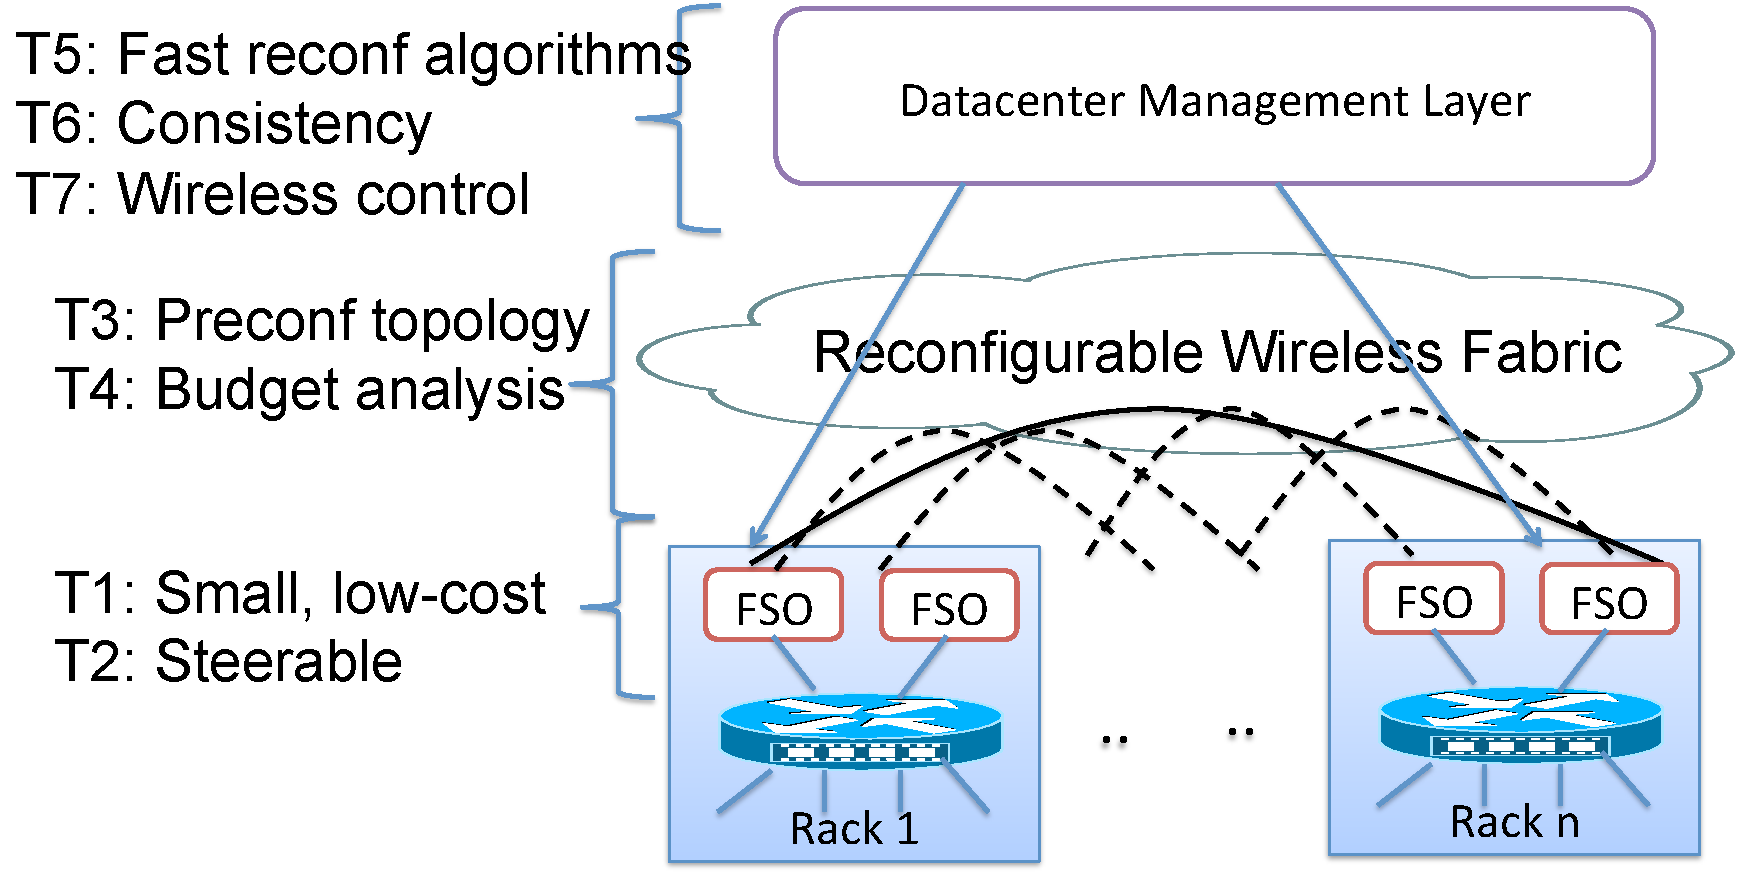
\includegraphics[width=220pt]{PPTFigs/introview_temp.pdf}
\caption{Overview of the \ArchName vision}
\label{fig:vision}
\end{wrapfigure}


%% vision .. extreme point, lots of benefits etc 
\mypara{Our vision}  In this proposed research, we consider an {\em extreme}
design point.  Instead of trying to incrementally improve the poor
cost-performance tradeoffs,  high  cabling complexity, and limited flexibility
of current \DC architectures, we envision a \emph{flexible}, {\em all-wireless}
inter-rack fabric.  
 
Figure~\ref{fig:vision} shows a conceptual overview of our vision called
\ArchName.\footnote{\ArchName  stands for \ArchNameExpand.} Each top-of-rack
(\ToR) switch has {\em flexible} wireless links that can be reconfigured to
connect  to other \ToRs.  The \DC management layer  reconfigures the  topology
to  adapt to  current traffic workloads. This vision offers several benefits
that current \DC architectures do not offer (\Section\ref{sec:motivation}).
First, topological flexibility (if done right)  provides a low-cost solution
(e.g., fewer switches, links) that obviates the need for overprovisioning.
Second, by virtue of being wireless, \ArchName eliminates cabling complexity
and attendant operational overheads (e.g., obstructed cooling)~\cite{hp-cable}
altogether. Third, this vision  can facilitate new and radical \DC topology
structures  that would otherwise remain ``paper designs'' due to cabling
complexity~\cite{jellyfish}.  Finally, flexibility can reduce energy
costs~\cite{googleisca,elastictree} and can enable administrators
 to   incrementally 
expand the \DC infrastructure to add more racks and machines as needed~\cite{jellyfish}.  

%\samir{This para needs to be rephrased, seems to repeat concepts.}

\mypara{Research plan and Intellectual Merit} To realize the all-wireless
vision outlined above, however, we need to look beyond traditional
\blue{radio-frequency (RF) based (e.g., 60GHz)} wireless solutions as they are
fundamentally constrained in terms of  range, capacity, and interference.   To
this end,  we rely on {\em Free-Space Optical communications} (FSO) as it can
offer very high data rates (tens of Gbps) over long ranges
($\approx$100m) using low
transmission power and with  low interference footprint.

 %\vyas{probably missing some segue on what makes this hard?}
 The unique characteristics of our approach---FSO-based inter-rack links,
all-wireless, and topology flexibility---raises novel algorithmic, networking,
and system-level challenges along three thrusts (Figure~\ref{fig:vision}): 

% in order to turn it into reality. 

\begin{packeditemize}

\item Datacenter scale deployments  impose new form-factor, cost, and
steerability requirements for FSOs that are fundamentally different from
their traditional long-haul use-cases.  Thus, we need  to develop
cost-effective solutions (\taskref{task:fso:sfp}) that can  be steered 
 at fine-grained timescales(\taskref{task:fso:steer}).

\item We need new algorithmic foundations to 
reason about flexible network design (\taskref{task:topology:dbw}).
Furthermore,  the  physical and geometric constraints of the steering
mechanisms raise new challenges for architecting the \DC subject to budget
constraints (\taskref{task:topology:preconf}).

\item Our vision imposes new network management challenges as well. In
particular, we need  novel algorithms for joint  topology
reconfiguration and traffic engineering
(\taskref{task:system:fastalgo}),  new  consistency abstractions that
guarantee connectivity  and performance when links may be in flux
(\taskref{task:system:dataplane}). Furthermore, we need new mechanisms
to replace  traditional wired control channels
(\taskref{task:system:ctrlchannel}).
 
%\item Proof-of-concept testbed

\end{packeditemize}


   %As discussed above, the proposed research spans
%aspects of optical technologies, electrical and mechanical steering solutions,
%algorithmic foundations of networking, wireless networks, and network
%management. 
\mypara{Team Qualifications} Our team comprising three computer scientists and
one mechanical engineer has complementary  expertise spanning the domains of
network algorithmics~\cite{},  wireless networking~\cite{}, network
management~\cite{}, software-defined networking~\cite{}, and laser-based
optical technologies~\cite{}. Thus, our team is  uniquely positioned to tackle the
aforementioned challenges.    The PIs have an established history of
collaboration~\cite{} and outreach activities~\cite{}, and the proposed  research will
further strengthen these existing collaborations.

%  and this research will continue in the same vein.
%
